\documentclass{article}
\usepackage[utf8]{inputenc}
\usepackage{graphicx}
\usepackage{booktabs}
\usepackage{float}
\graphicspath{ {./metrics/fold_0/} }
\graphicspath{ {./metrics/fold_1/} }
\graphicspath{ {./metrics/fold_2/} }
\title{Results: bert-base-uncased-lr-[0.0005|0.00001|0.000001]}
\author{Nadia Sheikh}
\date{2022-07-13}
\begin{document}
\maketitle
\section{Configurations}
\subsection{Run Configuration}
\begin{tabular}{ll}
\toprule
{} &                                                  0 \\
\midrule
experiment\_identifier        &                          llm-baseline-[bert|sbert] \\
run\_identifier               &     bert-base-uncased-lr-[0.0005|0.00001|0.000001] \\
max\_epochs                   &                                                  3 \\
loss\_functions               &                                 cross-entropy-loss \\
learning\_rates               &                         0.00005, 0.00001, 0.000005 \\
batch\_sizes                  &                                                  1 \\
optimizers                   &                                               adam \\
llm\_name                     &                                  bert-base-uncased \\
hidden\_dropout\_prob          &                                                0.1 \\
attention\_probs\_dropout\_prob &                                                0.1 \\
pooling\_strategy             &                                                cls \\
config\_file\_path             &  /tmp/71140.1.all.q/ctre/cnc-task-3/script-deve... \\
\bottomrule
\end{tabular}

\subsection{Data Configuration}
\begin{tabular}{ll}
\toprule
{} &                                                  0 \\
\midrule
data\_utility\_cls        &                                      cnc\_utilities \\
dataset\_cls             &                                   CNCTask3aDataset \\
nos\_of\_folds            &                                                  3 \\
trn\_data\_path           &    /cnc-task-3/script-development/data/CSV-Output/ \\
tst\_data\_path           &  /home/nadia/Documents/CLaC-Lab/ctre/cnc-task-3... \\
base\_output\_folder\_path &             /cnc-task-3/script-development/output/ \\
config\_file\_path        &  /tmp/71140.1.all.q/ctre/cnc-task-3/script-deve... \\
\bottomrule
\end{tabular}

\subsection{Preprocessing Configuration}
\begin{tabular}{ll}
\toprule
{} &                                                  0 \\
\midrule
collate\_fn\_name   &                                       LLMCollateFn \\
llm\_name          &                                  bert-base-uncased \\
connl\_folder\_path &  /home/nadia/Documents/CLaC-Lab/ctre/cnc-task-3... \\
max\_nos\_tokens    &                                                 84 \\
token\_sep         &                                               True \\
config\_file\_path  &  /tmp/71140.1.all.q/ctre/cnc-task-3/script-deve... \\
\bottomrule
\end{tabular}

\section{Hyperparameters}
\subsection{hparam\_config\_id\_0}
\begin{tabular}{ll}
\toprule
{} &                   0 \\
\midrule
loss\_function                &  cross-entropy-loss \\
learning\_rate                &             0.00005 \\
batch\_size                   &                   1 \\
optimizer                    &                adam \\
hidden\_dropout\_prob          &                 0.1 \\
attention\_probs\_dropout\_prob &                 0.1 \\
pooling\_strategy             &                 cls \\
\bottomrule
\end{tabular}

\subsection{hparam\_config\_id\_1}
\begin{tabular}{ll}
\toprule
{} &                   0 \\
\midrule
loss\_function                &  cross-entropy-loss \\
learning\_rate                &             0.00001 \\
batch\_size                   &                   1 \\
optimizer                    &                adam \\
hidden\_dropout\_prob          &                 0.1 \\
attention\_probs\_dropout\_prob &                 0.1 \\
pooling\_strategy             &                 cls \\
\bottomrule
\end{tabular}

\subsection{hparam\_config\_id\_2}
\begin{tabular}{ll}
\toprule
{} &                   0 \\
\midrule
loss\_function                &  cross-entropy-loss \\
learning\_rate                &            0.000005 \\
batch\_size                   &                   1 \\
optimizer                    &                adam \\
hidden\_dropout\_prob          &                 0.1 \\
attention\_probs\_dropout\_prob &                 0.1 \\
pooling\_strategy             &                 cls \\
\bottomrule
\end{tabular}

\section{fold\_0}
\subsection{train\_loss}
\begin{tabular}{lrrr}
\toprule
{} &   ep 0 &   ep 1 &   ep 2 \\
\midrule
hp\_0 &  0.809 &  0.751 &  0.713 \\
hp\_1 &  0.728 &  0.659 &  0.352 \\
hp\_2 &  0.710 &  0.672 &  0.474 \\
\bottomrule
\end{tabular}

\begin{figure}[H]
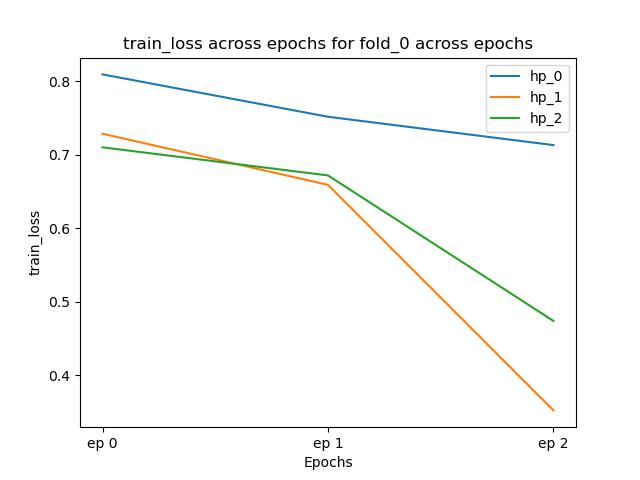
\includegraphics[scale = 0.75]{fold_0/train_loss}
\end{figure}
\subsection{test\_loss}
\begin{tabular}{lrrr}
\toprule
{} &   ep 0 &   ep 1 &   ep 2 \\
\midrule
hp\_0 &  0.694 &  0.689 &  0.623 \\
hp\_1 &  0.693 &  0.546 &  0.342 \\
hp\_2 &  0.701 &  0.612 &  0.476 \\
\bottomrule
\end{tabular}

\begin{figure}[H]
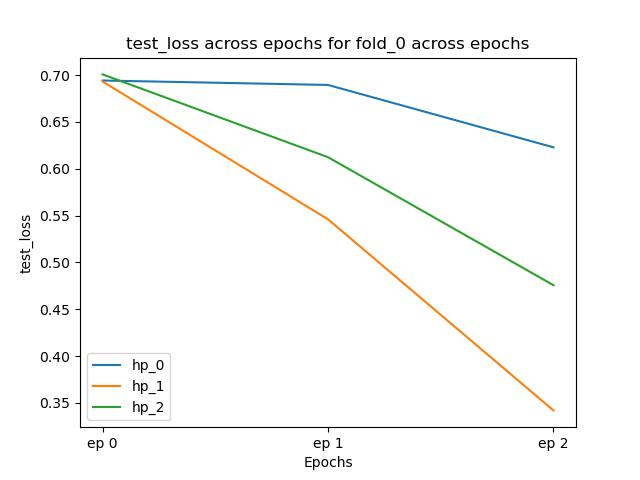
\includegraphics[scale = 0.75]{fold_0/test_loss}
\end{figure}
\subsection{accuracy\_score}
\begin{tabular}{lrrr}
\toprule
{} &   ep 0 &   ep 1 &   ep 2 \\
\midrule
hp\_0 &  0.470 &  0.521 &  0.778 \\
hp\_1 &  0.513 &  0.752 &  0.829 \\
hp\_2 &  0.556 &  0.675 &  0.786 \\
\bottomrule
\end{tabular}

\begin{figure}[H]
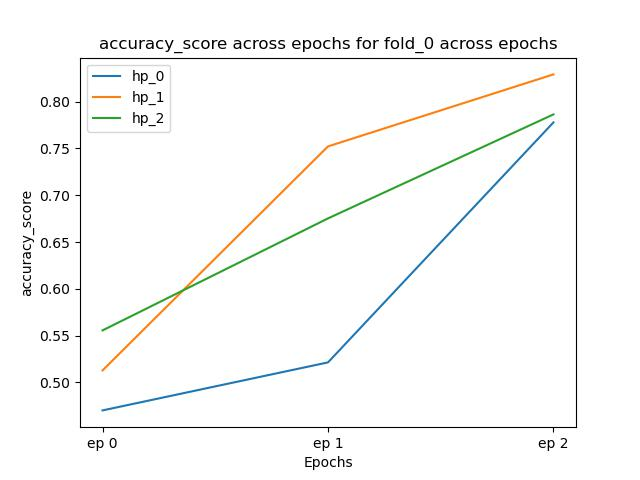
\includegraphics[scale = 0.75]{fold_0/accuracy_score}
\end{figure}
\subsection{f1\_score}
\begin{tabular}{lrrr}
\toprule
{} &   ep 0 &   ep 1 &   ep 2 \\
\midrule
hp\_0 &  0.640 &  0.000 &  0.806 \\
hp\_1 &  0.457 &  0.734 &  0.815 \\
hp\_2 &  0.671 &  0.596 &  0.762 \\
\bottomrule
\end{tabular}

\begin{figure}[H]
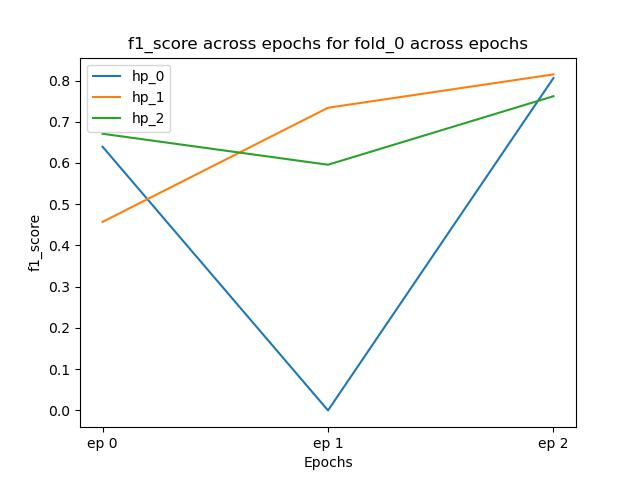
\includegraphics[scale = 0.75]{fold_0/f1_score}
\end{figure}
\subsection{precision\_score}
\begin{tabular}{lrrr}
\toprule
{} &   ep 0 &   ep 1 &   ep 2 \\
\midrule
hp\_0 &  0.474 &  0.000 &  0.692 \\
hp\_1 &  0.490 &  0.755 &  0.846 \\
hp\_2 &  0.520 &  0.737 &  0.816 \\
\bottomrule
\end{tabular}

\begin{figure}[H]
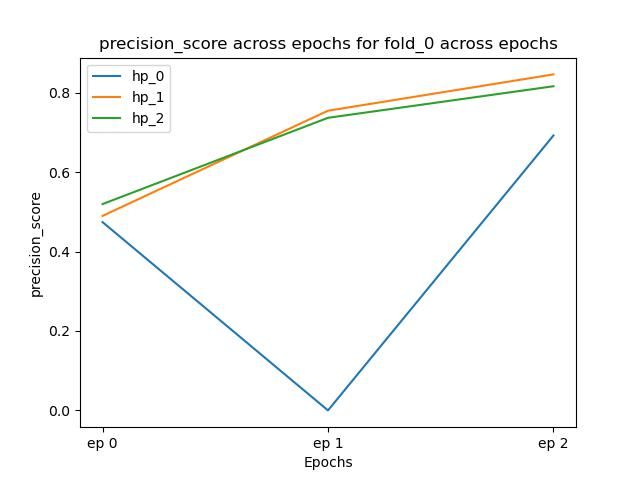
\includegraphics[scale = 0.75]{fold_0/precision_score}
\end{figure}
\subsection{matthews\_corrcoef}
\begin{tabular}{lrrr}
\toprule
{} &   ep 0 &   ep 1 &   ep 2 \\
\midrule
hp\_0 & -0.097 &  0.000 &  0.605 \\
hp\_1 &  0.019 &  0.503 &  0.658 \\
hp\_2 &  0.214 &  0.358 &  0.574 \\
\bottomrule
\end{tabular}

\begin{figure}[H]
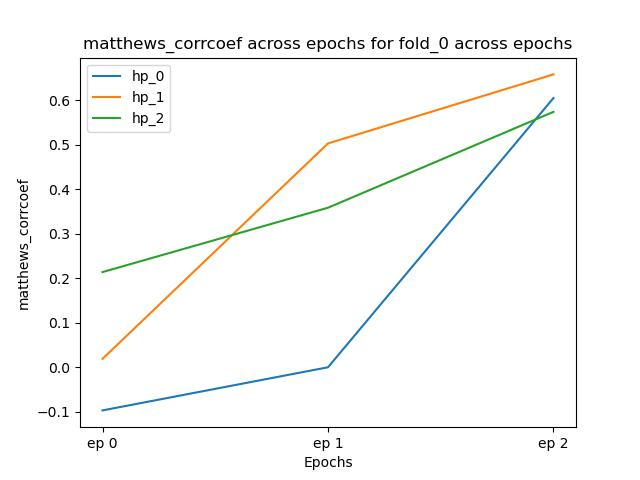
\includegraphics[scale = 0.75]{fold_0/matthews_corrcoef}
\end{figure}
\subsection{recall\_score}
\begin{tabular}{lrrr}
\toprule
{} &   ep 0 &   ep 1 &   ep 2 \\
\midrule
hp\_0 &  0.982 &  0.000 &  0.964 \\
hp\_1 &  0.429 &  0.714 &  0.786 \\
hp\_2 &  0.946 &  0.500 &  0.714 \\
\bottomrule
\end{tabular}

\begin{figure}[H]
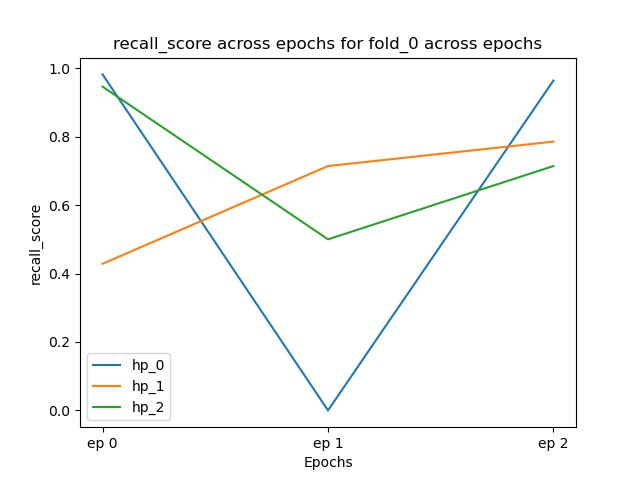
\includegraphics[scale = 0.75]{fold_0/recall_score}
\end{figure}
\section{fold\_1}
\subsection{train\_loss}
\begin{tabular}{lrrr}
\toprule
{} &   ep 0 &   ep 1 &   ep 2 \\
\midrule
hp\_0 &  0.787 &  0.705 &  0.475 \\
hp\_1 &  0.696 &  0.662 &  0.348 \\
hp\_2 &  0.710 &  0.678 &  0.456 \\
\bottomrule
\end{tabular}

\begin{figure}[H]
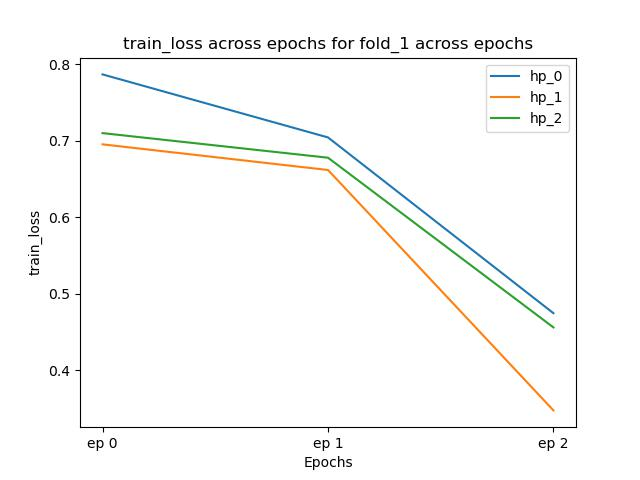
\includegraphics[scale = 0.75]{fold_1/train_loss}
\end{figure}
\subsection{test\_loss}
\begin{tabular}{lrrr}
\toprule
{} &   ep 0 &   ep 1 &   ep 2 \\
\midrule
hp\_0 &  0.706 &  0.647 &  0.393 \\
hp\_1 &  0.688 &  0.577 &  0.364 \\
hp\_2 &  0.714 &  0.641 &  0.458 \\
\bottomrule
\end{tabular}

\begin{figure}[H]
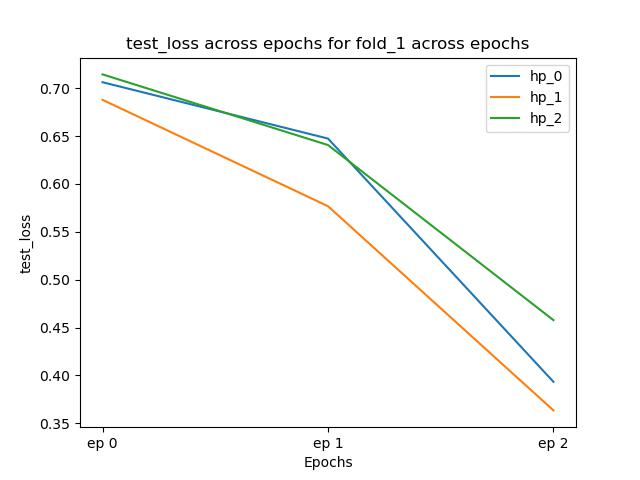
\includegraphics[scale = 0.75]{fold_1/test_loss}
\end{figure}
\subsection{accuracy\_score}
\begin{tabular}{lrrr}
\toprule
{} &   ep 0 &   ep 1 &   ep 2 \\
\midrule
hp\_0 &  0.457 &  0.638 &  0.819 \\
hp\_1 &  0.517 &  0.733 &  0.836 \\
hp\_2 &  0.448 &  0.621 &  0.793 \\
\bottomrule
\end{tabular}

\begin{figure}[H]
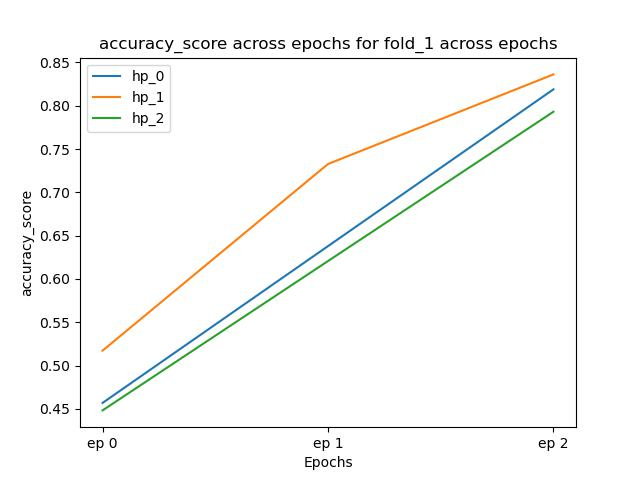
\includegraphics[scale = 0.75]{fold_1/accuracy_score}
\end{figure}
\subsection{f1\_score}
\begin{tabular}{lrrr}
\toprule
{} &   ep 0 &   ep 1 &   ep 2 \\
\midrule
hp\_0 &  0.000 &  0.533 &  0.807 \\
hp\_1 &  0.300 &  0.710 &  0.848 \\
hp\_2 &  0.467 &  0.500 &  0.800 \\
\bottomrule
\end{tabular}

\begin{figure}[H]
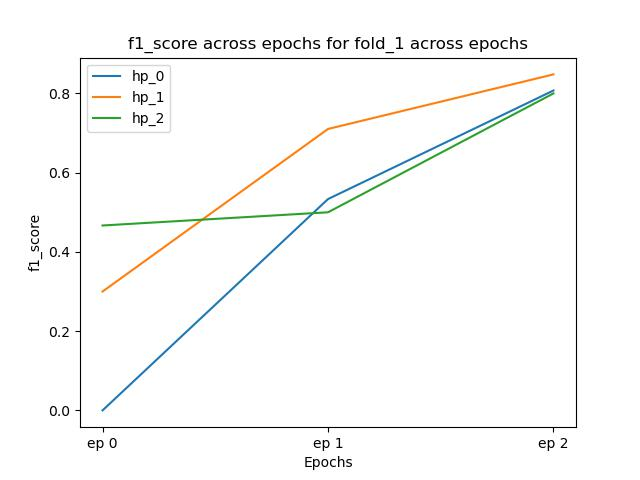
\includegraphics[scale = 0.75]{fold_1/f1_score}
\end{figure}
\subsection{precision\_score}
\begin{tabular}{lrrr}
\toprule
{} &   ep 0 &   ep 1 &   ep 2 \\
\midrule
hp\_0 &  0.000 &  0.857 &  0.936 \\
hp\_1 &  0.667 &  0.844 &  0.841 \\
hp\_2 &  0.483 &  0.846 &  0.828 \\
\bottomrule
\end{tabular}

\begin{figure}[H]
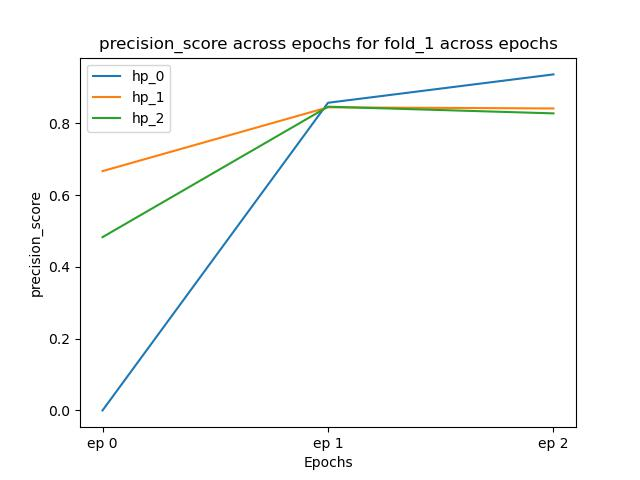
\includegraphics[scale = 0.75]{fold_1/precision_score}
\end{figure}
\subsection{matthews\_corrcoef}
\begin{tabular}{lrrr}
\toprule
{} &   ep 0 &   ep 1 &   ep 2 \\
\midrule
hp\_0 & -0.100 &  0.365 &  0.665 \\
hp\_1 &  0.114 &  0.495 &  0.671 \\
hp\_2 & -0.104 &  0.336 &  0.588 \\
\bottomrule
\end{tabular}

\begin{figure}[H]
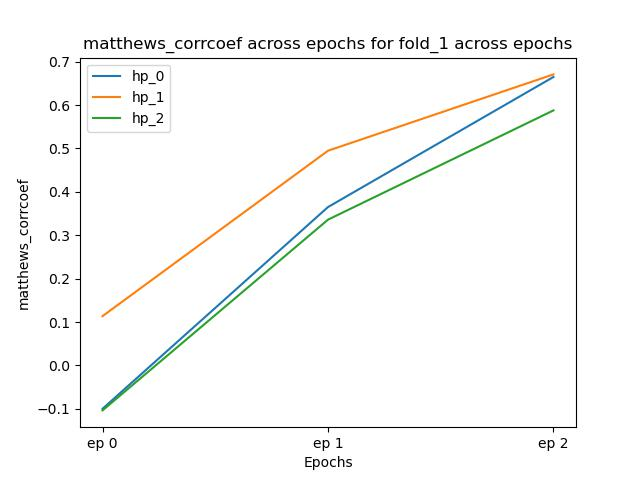
\includegraphics[scale = 0.75]{fold_1/matthews_corrcoef}
\end{figure}
\subsection{recall\_score}
\begin{tabular}{lrrr}
\toprule
{} &   ep 0 &   ep 1 &   ep 2 \\
\midrule
hp\_0 &  0.000 &  0.387 &  0.710 \\
hp\_1 &  0.194 &  0.613 &  0.855 \\
hp\_2 &  0.452 &  0.355 &  0.774 \\
\bottomrule
\end{tabular}

\begin{figure}[H]
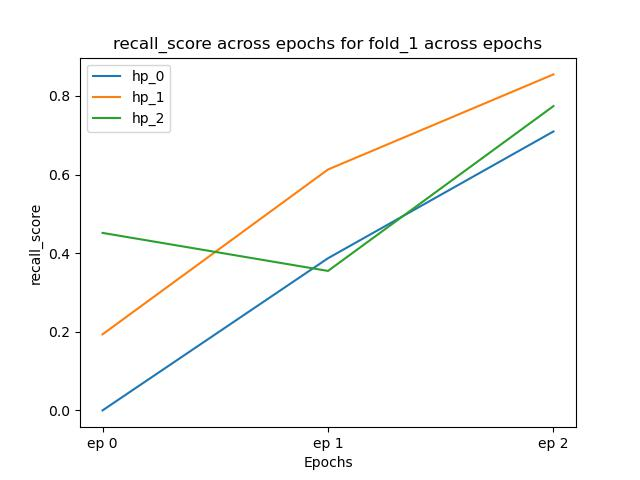
\includegraphics[scale = 0.75]{fold_1/recall_score}
\end{figure}
\section{fold\_2}
\subsection{train\_loss}
\begin{tabular}{lrrr}
\toprule
{} &   ep 0 &   ep 1 &   ep 2 \\
\midrule
hp\_0 &  0.767 &  0.692 &  0.542 \\
hp\_1 &  0.724 &  0.677 &  0.336 \\
hp\_2 &  0.710 &  0.689 &  0.512 \\
\bottomrule
\end{tabular}

\begin{figure}[H]
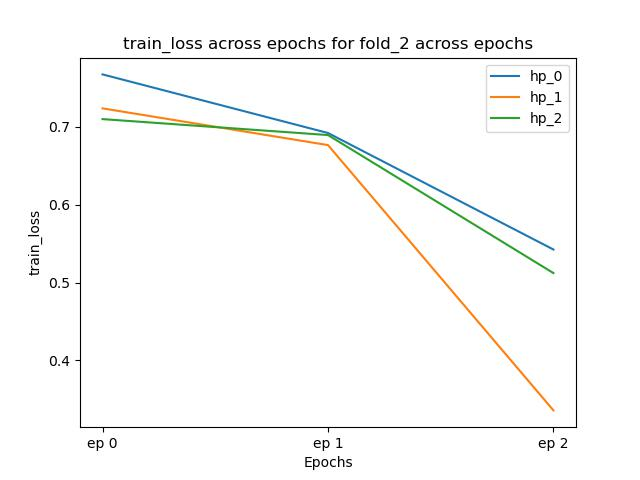
\includegraphics[scale = 0.75]{fold_2/train_loss}
\end{figure}
\subsection{test\_loss}
\begin{tabular}{lrrr}
\toprule
{} &   ep 0 &   ep 1 &   ep 2 \\
\midrule
hp\_0 &  0.694 &  0.633 &  0.610 \\
hp\_1 &  0.668 &  0.570 &  0.318 \\
hp\_2 &  0.706 &  0.600 &  0.443 \\
\bottomrule
\end{tabular}

\begin{figure}[H]
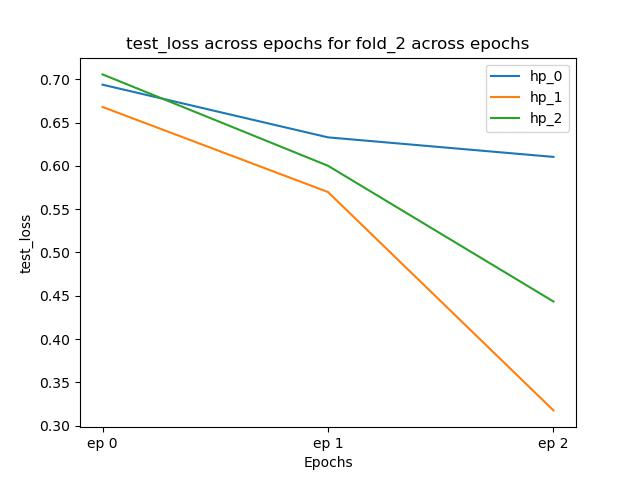
\includegraphics[scale = 0.75]{fold_2/test_loss}
\end{figure}
\subsection{accuracy\_score}
\begin{tabular}{lrrr}
\toprule
{} &   ep 0 &   ep 1 &   ep 2 \\
\midrule
hp\_0 &  0.491 &  0.724 &  0.724 \\
hp\_1 &  0.595 &  0.845 &  0.845 \\
hp\_2 &  0.491 &  0.750 &  0.853 \\
\bottomrule
\end{tabular}

\begin{figure}[H]
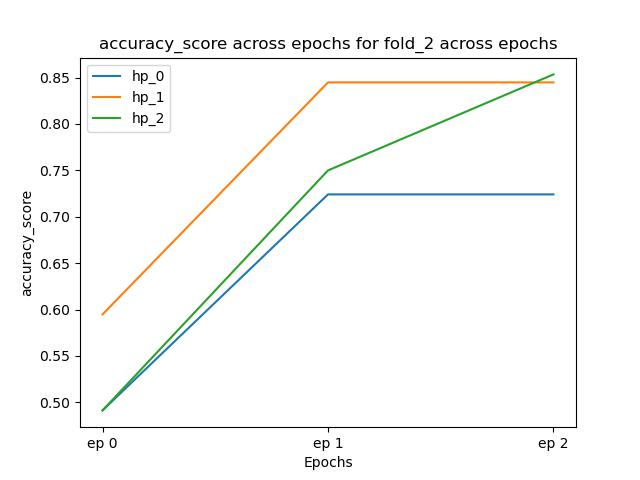
\includegraphics[scale = 0.75]{fold_2/accuracy_score}
\end{figure}
\subsection{f1\_score}
\begin{tabular}{lrrr}
\toprule
{} &   ep 0 &   ep 1 &   ep 2 \\
\midrule
hp\_0 &  0.604 &  0.742 &  0.742 \\
hp\_1 &  0.041 &  0.804 &  0.800 \\
hp\_2 &  0.587 &  0.701 &  0.821 \\
\bottomrule
\end{tabular}

\begin{figure}[H]
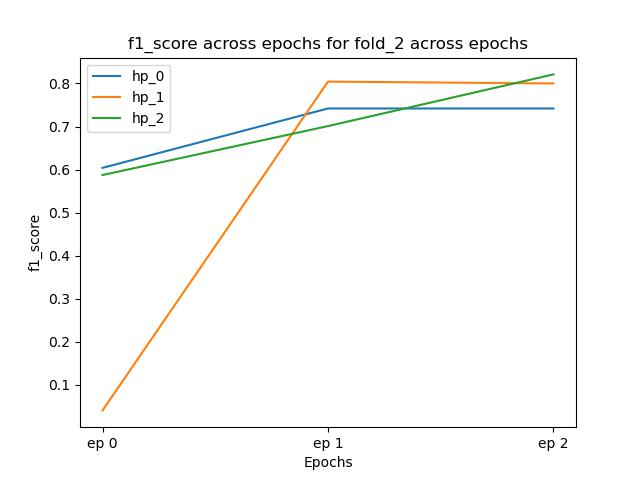
\includegraphics[scale = 0.75]{fold_2/f1_score}
\end{figure}
\subsection{precision\_score}
\begin{tabular}{lrrr}
\toprule
{} &   ep 0 &   ep 1 &   ep 2 \\
\midrule
hp\_0 &  0.446 &  0.605 &  0.605 \\
hp\_1 &  1.000 &  0.841 &  0.857 \\
hp\_2 &  0.442 &  0.694 &  0.830 \\
\bottomrule
\end{tabular}

\begin{figure}[H]
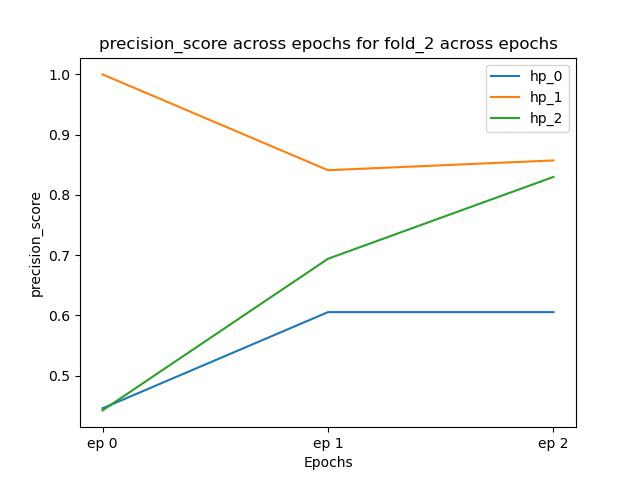
\includegraphics[scale = 0.75]{fold_2/precision_score}
\end{figure}
\subsection{matthews\_corrcoef}
\begin{tabular}{lrrr}
\toprule
{} &   ep 0 &   ep 1 &   ep 2 \\
\midrule
hp\_0 &  0.167 &  0.536 &  0.536 \\
hp\_1 &  0.111 &  0.678 &  0.678 \\
hp\_2 &  0.122 &  0.486 &  0.697 \\
\bottomrule
\end{tabular}

\begin{figure}[H]
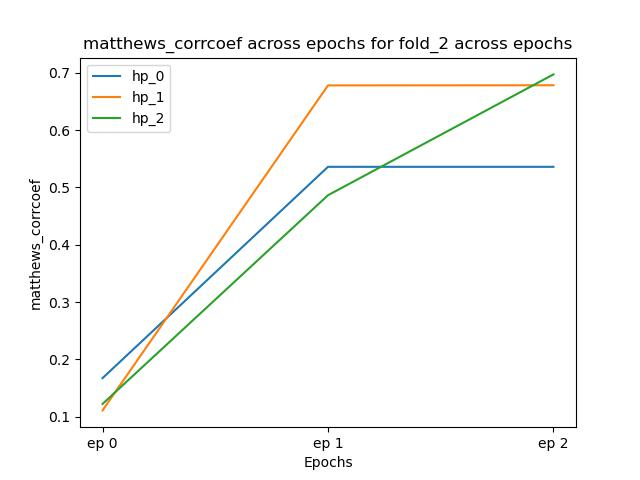
\includegraphics[scale = 0.75]{fold_2/matthews_corrcoef}
\end{figure}
\subsection{recall\_score}
\begin{tabular}{lrrr}
\toprule
{} &   ep 0 &   ep 1 &   ep 2 \\
\midrule
hp\_0 &  0.938 &  0.958 &  0.958 \\
hp\_1 &  0.021 &  0.771 &  0.750 \\
hp\_2 &  0.875 &  0.708 &  0.812 \\
\bottomrule
\end{tabular}

\begin{figure}[H]
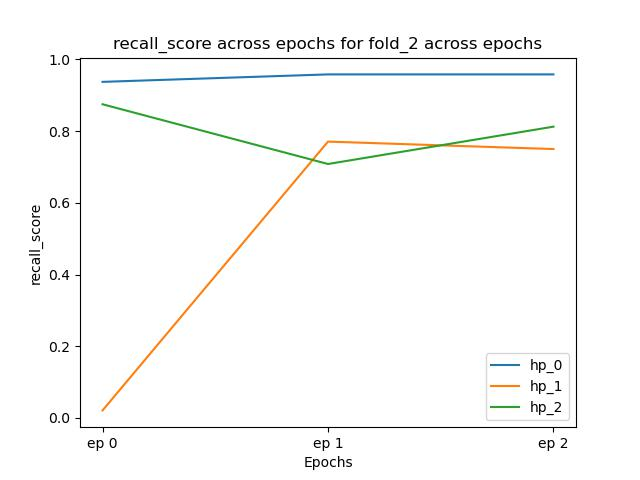
\includegraphics[scale = 0.75]{fold_2/recall_score}
\end{figure}
\end{document}
